\documentclass{article}

\PassOptionsToPackage{numbers,sort&compress}{natbib}

% Pass the exact package layout for RLJ format
\usepackage[accepted]{rlj}

% Core formatting and typography
\usepackage{microtype}
\usepackage{xcolor}

% Mathematical frameworks
\usepackage{amsmath,amssymb,amsthm,mathtools}
\usepackage{bm}
\usepackage{bbm}

% Layout structures
\usepackage{booktabs}
\usepackage{array}
\usepackage{enumitem}
\usepackage{graphicx}

% Summary and claim boxes
\usepackage[most]{tcolorbox}

% ---------------------------------------------------------------------
% Document Metadata & Running Headers
% ---------------------------------------------------------------------
\title{Why Is Manipulation Hard for Unsupervised RL?\\
A State-Based Diagnosis of Contact Bottlenecks in Cube Manipulation}

\setrunningtitle{A State-Based Diagnosis of Contact Bottlenecks in Cube Manipulation}

\author{%
  Aditya Mohan$^{1}$,
  Caleb Chuck$^{2}$,
  Siddhant Agarwal$^{2}$,
  Amy Zhang$^{2}$ \\
  $^{1}$Leibniz University Hannover, L3S Research Center \\
  $^{2}$University of Texas at Austin \\
  \texttt{a.mohan@ai.uni-hannover.de}
}

\emails{a.mohan@ai.uni-hannover.de}
\affiliations{}

% Figures path layout configuration
\graphicspath{{figure/}{figures/}}

% ---------------------------------------------------------------------
% Theorem-like environments & Style Blocks
% ---------------------------------------------------------------------
\newtheorem{proposition}{Proposition}
\newtheorem{definition}{Definition}
\newtheorem{hypothesis}{Hypothesis}
\newtheorem{remark}{Remark}

\tcbset{
    enhanced,
    sharp corners,
    boxrule=0.5pt,
    colback=white,
    colframe=black,
    coltitle=black,
    colbacktitle=white,
    fonttitle=\bfseries,
    left=1.5mm,
    right=1.5mm,
    top=1mm,
    bottom=1mm,
    before skip=8pt,
    after skip=8pt
}

\newtcolorbox{claimbox}[1]{title={#1}}

% ---------------------------------------------------------------------
% Mathematical Operators & Custom Macros
% ---------------------------------------------------------------------
\DeclareMathOperator*{\argmax}{arg\,max}
\DeclareMathOperator*{\argmin}{arg\,min}

\newcommand{\Sspace}{\mathcal{S}}
\newcommand{\Aspace}{\mathcal{A}}
\newcommand{\Ptrans}{P}
\newcommand{\R}{\mathbb{R}}
\newcommand{\E}{\mathbb{E}}
\newcommand{\Prob}{\mathbb{P}}
\newcommand{\ind}{\mathbf{1}}

\newcommand{\sm}{M^{\pi}}
\newcommand{\smz}{M^{\pi_z}}
\newcommand{\gciql}{\textsc{GCIQL}}
\newcommand{\fb}{\textsc{FB}}
\newcommand{\crl}{\textsc{crl}}
\newcommand{\psm}{\textsc{psm}}
\newcommand{\dreamer}{\textsc{MBRL}}
\newcommand{\ogbench}{\textsc{OGBench}}
\newcommand{\task}{\texttt{cube-single}}
\newcommand{\todo}[1]{\textbf{[TODO: #1]}}
\newcommand{\pp}{\mathrm{pp}}

% ---------------------------------------------------------------------
% Main Document Layout
% ---------------------------------------------------------------------
\begin{document}

\maketitle

\begin{abstract}
Many reinforcement learning domains are multi-task under a shared set of dynamics. 
Unsupervised reinforcement learning (URL) methods exploit this structure by pretraining without task rewards, then using the learned representation for downstream policy inference. 
Contact-rich manipulation is a challenging setting for this paradigm because future reachability depends on contact: IN sube manipulation tasks, this amounts to moving to the cube, acquiring a grasp, maintaining the grasp, and transporting the object induce different control regimes. 
This paper investigates whether state-based URL failures in cube manipulation are explained by this phase structure. 
We formalize manipulation as a phase-conditioned successor-measure problem and introduce a rollout diagnostic that assigns each failure to the first unmet physical precondition: approach, grasp, maintain grasp, or transport. On \ogbench{} \task{}, \gciql{} achieves higher aggregate success than \fb{}, but the decomposition reveals the relevant failure mode. 
\fb{} reaches the cube in all analyzed rollouts and has fewer initial grasp failures than \gciql{}, while most of the gap appears after pick-up through grasp-maintenance and transport failures. 
These results suggest that state-based manipulation failures in URL are not primarily failures of reaching the object, but failures to preserve phase-conditioned controllability after contact.
\end{abstract}

\section{Introduction}

One of the central promises of Unsupervised reinforcement learning (URL) is reusable-control: an agent first learns a task-agnostic representation of the environment, then uses it to solve multiple downstream tasks. 
In robotics, for example, a robot may need to solve many downstream goals in the same workspace, each specified by a different reward function. Learning a new policy from scratch for every reward can be prohibitively expensive. 
URL addresses this problem by first learning a representation, policy family, or value structure in a reward-free environment, and then using this object to infer policies for downstream rewards.

A wide range of URL algorithms instantiate this idea. 
Goal-conditioned methods learn policies or values conditioned on target states \citep{eysenbach2021clearning,ma2022offlinegcrl,park2025ogbench}. 
Contrastive RL methods learn representations that separate future states from negatives \citep{eysenbach2022contrastive,wang2023quasimetric,park2024hilp}. 
Successor-feature based methods learn reward-free objects that make downstream policy inference tractable \citep{dayan1993,barreto2017,touati2021,touati2023}. 
Proto-successor measures, proto-value functions, skill-discovery methods, controllable representations, and world models make different assumptions about what should be represented during pretraining \citep{mahadevan2005,mahadevan2007,farebrother2023,eysenbach2022infogeo,agarwal2025psm,efroni2022,lamb2022,levine2024,rudolph2024,hafner2020dreamer,hafner2023dreamerv3}. Although these methods use different losses and inference rules, many of them reason about future state occupancy, state reachability, or action-dependent predictability in some form \citep{agarwal2025unified}.

An often underexplored area for such methods has been the domain of manipulation.
Cube manipulation is not merely navigation in a larger state space. 
Moving a gripper to a cube, closing around it, lifting it, maintaining contact, and transporting it to a goal are different regimes of control. 
The transition between regimes is mediated by contact. 
Before grasp, gripper motion and object motion are weakly coupled; after grasp, they are tightly coupled; after a drop, the system returns to a different controllability regime. 
A representation that captures coarse reachability can therefore be inadequate if it fails to preserve which phase the system is in and which actions maintain control of the object.

This paper investigates the failure mode of state-based URL policies in contact-rich cube manipulation.
We use manipulation as a diagnostic domain for understanding what existing representations preserve and what they miss. 
Aggregate success is insufficient for this purpose. 
A policy that never reaches the cube, a policy that reaches but cannot lift, and a policy that lifts but cannot maintain contact all receive the same final failure label, even though they fail for different algorithmic reasons.

% Main idea: The hypothesis is phase-conditioned reachability.
\begin{hypothesis}[Contact bottleneck hypothesis]
Manipulation is hard for URL because the downstream task is not a single smooth reachability problem. It is a phase-conditioned control problem in which contact states act as bottlenecks. URL methods that compress future reachability without preserving contact phase may represent broad state reachability while failing to preserve the controllability needed for grasp maintenance and object transport.
\end{hypothesis}

% Main idea: Contributions separate the formal diagnosis, the empirical protocol, and the empirical finding.
We present the diagnosis in three steps.
\begin{enumerate}
    \item We formulate manipulation as a phase-conditioned successor-measure problem and define a phase-consistency condition for state abstractions. This makes precise how phase-blind compression can become successor-inconsistent around contact bottlenecks.
    \item We introduce a state-only failure decomposition for \ogbench{} \task{}. Each rollout is assigned to the first failed physical precondition: approach, grasp, maintain grasp, or transport.
    \item We apply this diagnostic to \fb{} and \gciql{}. \fb{} reaches the cube in all analyzed rollouts and has fewer initial grasp failures than \gciql{}, but its aggregate deficit is concentrated after pick-up. Pre-grasp and support diagnostics further indicate that the issue is not simply contact acquisition or nearest-neighbor dataset coverage.
\end{enumerate}

\section{Related Work}

\paragraph{Unsupervised reinforcement learning.}
URL methods pretrain in a reward-free or reward-agnostic phase and reuse the learned object for downstream control. Goal-conditioned RL learns policies or values indexed by target states \citep{eysenbach2021clearning,ma2022offlinegcrl}. Contrastive RL learns state-goal representations using future-positive and random-negative samples \citep{eysenbach2022contrastive}. Forward--backward representations and successor features estimate objects related to future occupancy and use them for reward-conditioned policy inference \citep{dayan1993,barreto2017,touati2021,touati2023}. Recent work has argued that many of these objectives are different tractable approximations to successor measures and that their representations induce state equivalences over future reachability \citep{agarwal2025unified}. Our work uses this perspective to analyze a concrete failure mode in manipulation rather than to derive a new URL objective.

\paragraph{Controllable representations.}
Controllable-representation methods learn abstractions that preserve action-relevant information, often through inverse or multi-step inverse dynamics objectives \citep{efroni2022,lamb2022,levine2024,rudolph2024}. These objectives are closely related to manipulation because contact changes which components of the state are controllable by the robot. We do not introduce a new controllability objective. Instead, we test whether existing state-based URL methods preserve the phase distinctions that such objectives would ideally retain.

\paragraph{Manipulation benchmarks and diagnostics.}
\ogbench{} provides offline goal-conditioned RL tasks that evaluate long-horizon control and goal reaching \citep{park2025ogbench}. Benchmark success rates are useful for comparing methods, but they do not identify the physical stage at which a policy fails. Our diagnostic decomposes manipulation rollouts into approach, grasp, maintain-grasp, and transport outcomes. This separates failures before contact, failures in contact acquisition, and failures after the object should have become controllable.

\section{Problem Setting and Background}
\label{sec:background}

\subsection{Reward-free pretraining and successor measures}

% Main idea: Define the reward-free MDP and successor measure used throughout the paper.
We consider a reward-free Markov decision process $(\Sspace,\Aspace,\Ptrans,\gamma)$ with state space $\Sspace$, action space $\Aspace$, transition kernel $\Ptrans$, and discount factor $\gamma$. For a policy $\pi$, the successor measure from $(s,a)$ to a measurable set $X\subseteq \Sspace$ is
\begin{equation}
    M^{\pi}(s,a,X)
    =
    \E_{\pi}\left[
        \sum_{t\geq 0}\gamma^t\ind\{s_{t+1}\in X\}
        \mid s_0=s,a_0=a
    \right].
\end{equation}
When the state space is discrete, we write $M^{\pi}(s,a,s^+)$ for the discounted occupancy of state $s^+$.

% Main idea: Successor measures turn reward-conditioned policy evaluation into a linear objective.
For a state reward $r$, policy evaluation can be written as
\begin{equation}
    Q^{\pi}_r(s,a)
    =
    \int_{\Sspace} M^{\pi}(s,a,ds^+) r(s^+).
\end{equation}
This identity explains why successor measures are useful for URL: a reward-free object that predicts future occupancy can be combined with a downstream reward to evaluate or infer policies \citep{touati2021,touati2023,agarwal2025unified}.

% Main idea: Practical methods compress the successor object; this creates the relevant risk.
The exact successor measure is intractable to represent for a large policy class. Practical URL methods therefore impose parametric structure. \fb{} uses a low-rank approximation,
\begin{equation}
    M^{\pi_z}(s,a,s^+)
    \approx
    F(s,a,z)^{\top}B(s^+),
\end{equation}
where $z$ indexes a reward or policy embedding \citep{touati2021,touati2023}. Goal-conditioned and contrastive methods use target-conditioned values, policies, or embeddings instead of explicitly representing the full measure \citep{eysenbach2021clearning,eysenbach2022contrastive,ma2022offlinegcrl}. \psm{} and related basis methods approximate successor or value objects through learned bases \citep{mahadevan2005,mahadevan2007,farebrother2023,agarwal2025psm}. In each case, the representation must decide which states are equivalent for downstream control.

\subsection{Manipulation as phase-conditioned reachability}

% Main idea: Contact phase changes the transition kernel.
We model a manipulation state as
\begin{equation}
    s=(x,o,g,c),
\end{equation}
where $x$ denotes robot proprioception, $o$ denotes object pose, $g$ denotes goal pose, and $c$ denotes a contact phase. The phase variable may be latent in the observation, but it changes how actions affect the object. We write the transition kernel as
\begin{equation}
    P(s'\mid s,a)
    =
    P_c(x',o',c'\mid x,o,c,a).
\end{equation}
For cube manipulation, the relevant phases include free approach, contact acquisition, stable grasped transport, unstable contact, and dropped contact.

% Main idea: Geometric proximity and controllability are different.
This formulation separates geometric proximity from controllability. When the cube is not grasped, actions that move the gripper need not move the cube. When the cube is stably grasped, similar gripper actions transport the cube. When contact is lost, the same object-goal distance can correspond to a different set of feasible future trajectories. As a result, a representation that preserves only object-goal geometry may merge states whose future occupancy of successful transport states is different.

\section{Phase-Conditioned Successor Diagnosis}
\label{sec:theory}

\subsection{Phase consistency}

% Main idea: A safe abstraction must preserve successor measures for the policy class of interest.
We use successor consistency to state the representation requirement induced by contact.

\begin{definition}[Phase-consistent successor abstraction]
An abstraction $\phi:\Sspace\to\mathcal{Z}$ is phase-consistent for a policy class $\Pi$ if $\phi(s_1)=\phi(s_2)$ implies
\begin{equation}
    M^{\pi}(s_1,a,X)
    =
    M^{\pi}(s_2,a,X),
    \qquad
    \forall \pi\in\Pi,\; a\in\Aspace,\; X\subseteq\Sspace.
\end{equation}
\end{definition}

% Main idea: This condition is stronger than preserving object-goal distance.
The definition is stronger than preserving distances in the observed state. It requires preserving whether the cube is controllable, whether the grasp is stable, and whether future actions keep the system in a phase from which transport is possible. In contact-rich domains, these properties can change discontinuously at grasp, slip, and drop events.

\subsection{Contact bottlenecks create successor inconsistency}

% Main idea: A simple proposition shows why phase-blind abstraction can fail.
\begin{proposition}[Phase-blind abstractions fail at contact bottlenecks]
Consider a two-phase manipulation MDP with contact phase $c\in\{0,1\}$ and target set
\begin{equation}
    G=\{s:c=1,\|o-g\|\leq\epsilon\}.
\end{equation}
Suppose two states $s_1=(x_1,o,g,0)$ and $s_2=(x_2,o,g,0)$ have identical object and goal coordinates but differ in the probability of entering the grasped phase under some policy $\pi$:
\begin{equation}
    \Prob_{\pi}(\tau_{c=1}<\infty\mid s_1,a)
    \neq
    \Prob_{\pi}(\tau_{c=1}<\infty\mid s_2,a).
\end{equation}
Then any abstraction $\phi$ that ignores the variables responsible for this difference and maps $\phi(s_1)=\phi(s_2)$ is not successor-consistent for $G$.
\end{proposition}

\begin{proof}[Proof sketch]
Reaching $G$ requires entering the grasped phase. Therefore,
\begin{equation}
    M^{\pi}(s_i,a,G)
    =
    \E_{\pi}\left[
        \gamma^{\tau_{c=1}}
        M^{\pi}(s_{\tau_{c=1}},a_{\tau_{c=1}},G)
        \ind\{\tau_{c=1}<\infty\}
        \mid s_i,a
    \right].
\end{equation}
If the probability or timing of entering $c=1$ differs between $s_1$ and $s_2$, the successor mass assigned to $G$ differs unless later transport dynamics exactly cancel the difference. Such cancellation is not generic. Thus $M^{\pi}(s_1,a,G)\neq M^{\pi}(s_2,a,G)$, contradicting successor consistency.
\end{proof}

% Main idea: This proposition motivates phase-level evaluation.
The proposition gives a concrete interpretation of manipulation failures. A representation may be useful for broad reachability and still fail if it merges states that differ in contact acquisition, grasp stability, or transport controllability. The empirical protocol therefore measures the physical phase at which each rollout first fails.

\subsection{Predictions for URL methods}

% Main idea: Different method families should exhibit different phase-level failures.
The phase-conditioned view gives method-specific predictions. Goal-conditioned value methods such as \gciql{} can succeed when the dataset contains enough bottleneck-crossing trajectories and the value function assigns correct credit to actions that preserve contact \citep{ma2022offlinegcrl,kostrikov2022iql,park2025ogbench}. Contrastive methods may learn useful reachability geometry, but representation-space closeness to the goal does not guarantee that the policy can cross a contact bottleneck \citep{eysenbach2022contrastive}. \fb{} can retarget rewards through a compact successor factorization, but a single low-rank embedding $z=B(g)$ may allocate insufficient capacity to the distinction between approach, grasp, and transport \citep{touati2021,touati2023}. \psm{} provides a basis-coverage diagnostic: if no proto-policy occupies stable grasped transport, downstream inference cannot easily synthesize reliable transport from the basis \citep{agarwal2025psm}. A model-based method provides an orthogonal diagnostic: if imagined rollouts do not predict lift, slip, or drop transitions, planning fails at the same boundary \citep{hafner2020dreamer,hafner2023dreamerv3}.

\section{Diagnostic Method}
\label{sec:method}

\subsection{Evaluation setting}

% Main idea: Completed experiments compare FB and GCIQL on state-based OGBench cube-single.
We study the state-observation version of \ogbench{} \task{} over five held-out evaluation tasks, denoted \textit{task1}--\textit{task5}. The completed comparison is between \fb{} and \gciql{}. \fb{} learns a forward--backward successor factorization with a behavior-regularized actor. \gciql{} is the goal-conditioned IQL-style baseline used in the \ogbench{} reference implementation. We report interquartile mean (IQM) success with stratified-bootstrap confidence intervals for aggregate performance. We then analyze deterministic closed-loop rollouts using the phase decomposition below.

\subsection{Phase decomposition}

% Main idea: Each episode receives the earliest failed physical precondition as its terminal label.
Each rollout is assigned to exactly one terminal outcome: success, or the first failed phase in the ordered manipulation pipeline. The ordered phases are approach, grasp, maintain grasp, and transport. A transport failure is therefore counted only if the rollout has already satisfied the approach and grasp criteria.

\begin{table}[h]
\centering
\caption{Operational criteria for assigning the first failure phase in state rollouts.}
\label{tab:failure_criteria}
\begin{tabular}{ll}
\toprule
\textbf{Phase} & \textbf{Criterion} \\
\midrule
Approach & Minimum gripper-to-cube distance $<6$ cm at any point in the episode \\
Grasp & Cube lifted $>3$ cm above table with gripper closed for at least $5$ consecutive steps \\
Maintain grasp & Final cube height above table $\geq 3$ cm \\
Transport & Final cube pose within $5$ cm of the goal pose \\
\bottomrule
\end{tabular}
\end{table}

% Main idea: The decomposition is method-agnostic.
The criteria in Table~\ref{tab:failure_criteria} are mechanical and policy-agnostic. They do not use the value function, the learned representation, or any method-specific internal score. This makes the same evaluation applicable to goal-conditioned, contrastive, successor-measure, and model-based methods.

\subsection{Intervention and representation diagnostics}

% Main idea: The additional diagnostics distinguish contact acquisition, support, and terminal resolution.
The phase decomposition identifies where a rollout fails. 
We add three diagnostics to test why the failure occurs. 
First, a pre-grasp intervention initializes the cube inside the gripper. If the main bottleneck is only entering the grasped state, this intervention should improve success. 
Second, a nearest-neighbor support diagnostic compares successful and failed states to similar states in the offline dataset. 
If transport failure is primarily an out-of-distribution effect, failed transport states should have much larger nearest-neighbor distances. 
Third, two \fb{} diagnostics test whether the learned value and backward embedding provide goal-directed terminal resolution: a Spearman correlation between value and negative cube-goal distance, and probes from $B(s)$ to cube-goal distance and placed-versus-near-miss labels.

\section{Results}
\label{sec:results}

\subsection{Aggregate state success shows a gap}

% Main idea: Aggregate success motivates the diagnosis but does not explain the failure mechanism.
Table~\ref{tab:overall_state} reports aggregate state-based success. \gciql{} outperforms \fb{} overall, with an IQM of $68.3\%$ compared to $50.0\%$ for \fb{}. This result motivates the diagnosis, but does not by itself identify whether \fb{} fails before contact, during contact acquisition, or after the cube is lifted.

\begin{table}[h]
\centering
\caption{State-based evaluation performance. Values are IQM $\pm$ half-width of the $95\%$ stratified-bootstrap confidence interval across seeds.}
\label{tab:overall_state}
\begin{tabular}{lcccccc}
\toprule
\textbf{Method} & \textbf{task1} & \textbf{task2} & \textbf{task3} & \textbf{task4} & \textbf{task5} & \textbf{Overall} \\
\midrule
\fb{}    & $16.7 \pm 10.0$ & $68.3 \pm 10.9$ & $75.0 \pm 10.0$ & $40.0 \pm 13.3$ & $43.3 \pm 18.4$ & $\mathbf{50.0 \pm 7.0}$ \\
\gciql{} & $73.7 \pm 5.9$  & $70.0 \pm 7.0$  & $73.0 \pm 7.0$  & $58.0 \pm 5.2$  & $64.3 \pm 7.0$  & $\mathbf{68.3 \pm 3.7}$ \\
\bottomrule
\end{tabular}
\end{table}

\begin{figure}[h]
\centering
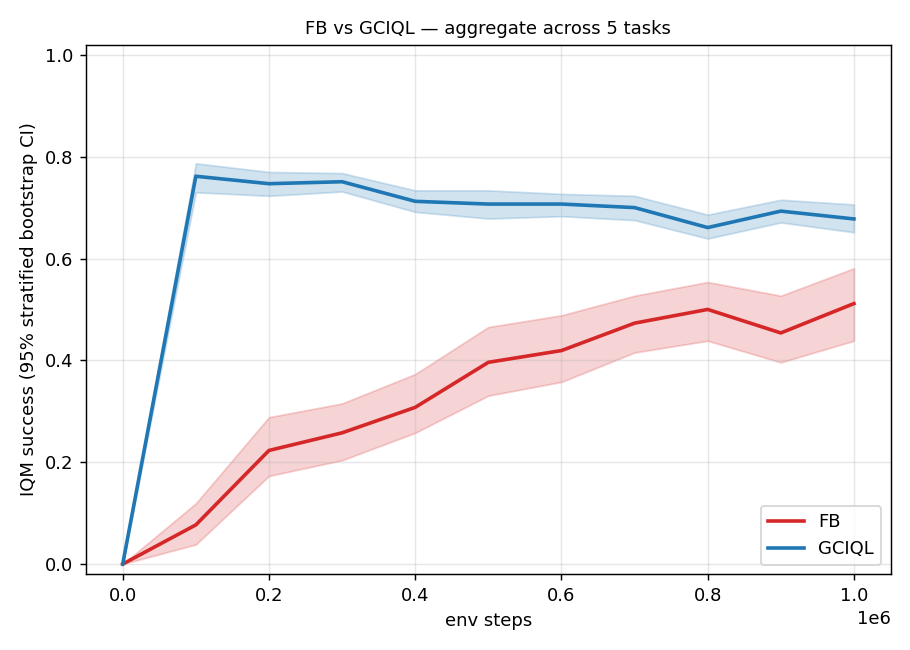
\includegraphics[width=0.85\linewidth]{f1_curves_aggregate}
\caption{Training-time IQM success on \task{} state observations for \fb{} and \gciql{}. The aggregate gap is established by mid-training and persists; per-task curves (Appendix) confirm the same ordering. Shaded regions are $95\%$ stratified-bootstrap confidence intervals across 10 seeds.}
\label{fig:training_curves}
\end{figure}

\subsection{\fb{} failures concentrate after pick-up}

% Main idea: FB reaches and grasps; its dominant failures are after lift.
Across $350$ \fb{} state rollouts, approach is solved under our operational criterion and initial grasp failures are relatively rare. The dominant failures occur after the cube has been lifted.

\begin{table}[h]
\centering
\caption{Outcome distribution for state-based \fb{} rollouts across $7$ seeds, $5$ tasks, and $10$ episodes per task.}
\label{tab:fb_state_outcomes}
\begin{tabular}{lcc}
\toprule
\textbf{Outcome} & \textbf{Mean (\% episodes)} & \textbf{Std} \\
\midrule
Success                          & $51.1$ & $10.8$ \\
Failure to approach              & $0.0$  & $0.0$ \\
Failure to grasp                 & $7.7$  & $3.4$ \\
Failure to maintain grasp        & $23.7$ & $9.9$ \\
Failure to transport to goal     & $17.4$ & $6.6$ \\
\bottomrule
\end{tabular}
\end{table}

% Main idea: The phase comparison localizes the FB-GCIQL gap.
Table~\ref{tab:state_decomp} compares \fb{} and \gciql{} under the same decomposition. The $18.1\pp$ success gap is not explained by approach. It is also not explained by initial grasp, where \fb{} has fewer failures under the operational criterion. The gap is concentrated in maintain-grasp and transport outcomes.

\begin{table}[h]
\centering
\caption{State-regime phase decomposition. Negative values in the final column indicate higher \fb{} failure or lower \fb{} success.}
\label{tab:state_decomp}
\begin{tabular}{lccc}
\toprule
\textbf{Outcome} & \textbf{\fb{} (\% eps)} & \textbf{\gciql{} (\% eps)} & \textbf{\fb{} $-$ \gciql{} (pp)} \\
\midrule
Success                          & $51.1$ & $69.2$ & $\mathbf{-18.1}$ \\
Failure to approach              & $0.0$  & $0.2$  & $-0.2$ \\
Failure to grasp                 & $7.7$  & $12.2$ & $+4.5$ \\
Failure to maintain grasp        & $23.7$ & $9.2$  & $\mathbf{-14.5}$ \\
Failure to transport to goal     & $17.4$ & $9.2$  & $\mathbf{-8.2}$ \\
\bottomrule
\end{tabular}
\end{table}

The gap decomposes as
\begin{equation}
    -18.1
    =
    -0.2_{\text{approach}}
    +4.5_{\text{grasp}}
    -14.5_{\text{maintain}}
    -8.2_{\text{transport}}.
\end{equation}
This is the main empirical finding. \fb{} does not primarily fail by missing the cube. It fails after contact should have made the object controllable.

% Main idea: Transport failures are not simply small errors near the target.
A near-miss analysis supports this interpretation. Across $350$ \fb{} state rollouts and $500$ \gciql{} state rollouts, there are no episodes in which the agent finishes while holding the cube within one $5$ cm success radius of the goal. The transport failures are therefore not fine placement errors near the target. They are failures to bring the held object into the target neighborhood.

\begin{figure}[h]
\centering
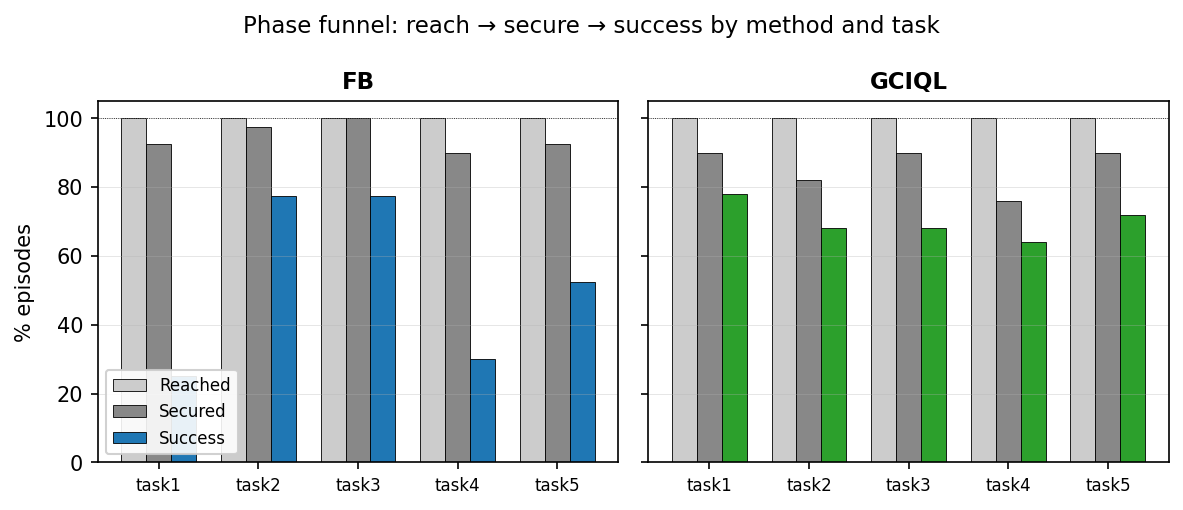
\includegraphics[width=0.92\linewidth]{f2_funnel_fbgciql}
\caption{Phase funnel by method and task: rate at which evaluation rollouts reach the cube (light grey), maintain a stable grasp at lift-off (dark grey), and terminate within $5$ cm of the goal (coloured). Reach is solved by both methods; \fb{}'s drop-off occurs between secure and success on tasks~$1$ and~$4$, while \gciql{}'s drop-off is distributed more evenly across the ladder. Rates are IQM over per-seed rollout rates ($10$ episodes per (seed, task), $7$ \fb{} seeds, $10$ \gciql{} seeds, scenario~S0); the protocol matches the IQM convention used for Table~\ref{tab:overall_state} but does not include the stratified-bootstrap CI half-widths.}
\label{fig:funnel}
\end{figure}

\subsection{Pre-grasping does not improve \fb{}}

% Main idea: Pre-grasping tests whether contact acquisition is the main bottleneck.
The pre-grasp intervention tests whether \fb{} mainly fails because it cannot enter the object-interaction regime. In this intervention, the cube is initialized inside the gripper. If the main bottleneck were contact acquisition, success should increase. Instead, success decreases.

\begin{table}[h]
\centering
\caption{\fb{} intervention study. S0 is the original evaluation, S1 is a sanity control, and S2 initializes the cube pre-grasped. Values are mean $\pm$ standard deviation across seeds.}
\label{tab:intervention}
\begin{tabular}{lccc}
\toprule
\textbf{Scenario} & \textbf{Reached} & \textbf{Secured} & \textbf{Success} \\
\midrule
S0 baseline    & $100.0 \pm 0.0$ & $92.3 \pm 3.4$ & $51.1 \pm 10.8$ \\
S1 control     & $100.0 \pm 0.0$ & $95.7 \pm 1.7$ & $50.0 \pm 8.3$  \\
S2 pre-grasped & $100.0 \pm 0.0$ & $85.1 \pm 8.7$ & $35.7 \pm 8.2$  \\
\bottomrule
\end{tabular}
\end{table}

The result in Table~\ref{tab:intervention} argues against a simple contact-acquisition explanation. Initializing the policy in the grasped regime does not make the controller reliably transport the cube. The policy must preserve the coupling between gripper and cube while steering the object to the goal.

\subsection{Dataset support does not explain the pattern}

% Main idea: Failed transport states are not obviously much farther from the offline data.
The support diagnostic does not indicate a simple out-of-distribution explanation. If transport failures were mainly caused by leaving the dataset manifold, failed transport states should have much larger nearest-neighbor distances than successful transport states. The differences in Table~\ref{tab:state_coverage} are small.

\begin{table}[h]
\centering
\caption{State observations: dataset-manifold support. $m_{\mathrm{dist}}$ is the nearest-neighbor distance to comparable states in the offline dataset; larger values indicate lower support.}
\label{tab:state_coverage}
\begin{tabular}{lcc}
\toprule
\textbf{Region} & \textbf{$m_{\mathrm{dist}}$ (Success)} & \textbf{$m_{\mathrm{dist}}$ (Transport-Fail)} \\
\midrule
reach     & $2.22 \pm 0.74$ & $2.41 \pm 1.29$ \\
lift      & $2.44 \pm 1.73$ & $2.54 \pm 1.41$ \\
transport & $2.12 \pm 0.79$ & $2.25 \pm 1.02$ \\
\bottomrule
\end{tabular}
\end{table}

This result does not show that support is irrelevant. Nearest-neighbor distance is a coarse statistic, and local action support may still differ between successful and failed rollouts. However, the observed transport failures do not appear to arise simply because failed states are far from the offline dataset.

\subsection{The \fb{} representation gives weak terminal guidance}

% Main idea: FB value does not monotonically guide the cube toward the goal.
We next test whether the learned \fb{} value provides a transport signal toward the goal. For each episode, we compute the Spearman correlation between the extracted value $V(s)=Q_z(s,\pi(s))$ and negative cube-to-goal distance $-d(s,g)$. A positive correlation means that value increases as the cube gets closer to the goal. The correlations in Table~\ref{tab:state_value_gradient} are weak for both successful and transport-failed episodes.

\begin{table}[h]
\centering
\caption{State observations: value-landscape gradient for \fb{}. Higher positive $\rho$ means value ranks states closer to the goal as better.}
\label{tab:state_value_gradient}
\begin{tabular}{lcc}
\toprule
\textbf{Task} & \textbf{$\rho$ (Success)} & \textbf{$\rho$ (Transport-Fail)} \\
\midrule
\textit{task1} & $0.258 \pm 0.264$ & $0.327 \pm 0.358$ \\
\textit{task2} & $0.089 \pm 0.341$ & $0.196 \pm 0.249$ \\
\textit{task3} & $0.163 \pm 0.332$ & $0.145 \pm 0.213$ \\
\textit{task4} & $0.113 \pm 0.664$ & $0.189 \pm 0.466$ \\
\textit{task5} & $0.112 \pm 0.568$ & $0.206 \pm 0.446$ \\
\midrule
\textbf{Mean} & $\mathbf{0.147}$ & $\mathbf{0.213}$ \\
\bottomrule
\end{tabular}
\end{table}

% Main idea: The backward representation only moderately resolves terminal placement.
The backward representation $B(s)$ also has limited terminal resolution. A ridge probe from $B(s)$ to cube-goal distance reaches moderate $R^2$, and a classifier separating true placements from close near-misses reaches only moderate accuracy.

\begin{table}[h]
\centering
\caption{State observations: $B$-embedding spatial resolution.}
\label{tab:state_b_resolution}
\begin{tabular}{lcc}
\toprule
\textbf{Task} & \textbf{Ridge $R^2(B\to d)$} & \textbf{Placed-vs-Near-Miss Acc.} \\
\midrule
\textit{task1} & $0.391 \pm 0.024$ & $0.635 \pm 0.023$ \\
\textit{task2} & $0.267 \pm 0.025$ & $0.678 \pm 0.016$ \\
\textit{task3} & $0.234 \pm 0.016$ & $0.681 \pm 0.016$ \\
\textit{task4} & $0.529 \pm 0.005$ & $0.664 \pm 0.018$ \\
\textit{task5} & $0.545 \pm 0.024$ & $0.668 \pm 0.014$ \\
\midrule
\textbf{Mean} & $\mathbf{0.393}$ & $\mathbf{0.665}$ \\
\bottomrule
\end{tabular}
\end{table}

Together, these diagnostics support the contact-bottleneck interpretation. The main issue is not just reaching the cube or entering contact. The representation and policy must distinguish states in which the cube is geometrically close, physically controlled, and stably transportable from states in which only some of these conditions hold.

\section{Extending the Protocol Across URL Methods}
\label{sec:extensions}

% Main idea: The evaluation labels are method-agnostic.
The state-only decomposition is not tied to \fb{} or \gciql{}. The same labels can be applied to \crl{}, \psm{}, and model-based methods without changing the evaluation protocol. The rows below separate completed measurements from planned diagnostics.

\begin{table}[h]
\centering
\caption{State-only cross-method diagnostic table. The \crl{} row should be filled from available state runs; \psm{} and \dreamer{} rows indicate planned diagnostics rather than completed empirical results.}
\label{tab:cross_method_template}
\begin{tabular}{lccccc}
\toprule
\textbf{Method} & \textbf{Success} & \textbf{Approach fail} & \textbf{Grasp fail} & \textbf{Maintain fail} & \textbf{Transport fail} \\
\midrule
\fb{}    & $51.1$ & $0.0$ & $7.7$  & $23.7$ & $17.4$ \\
\gciql{} & $69.2$ & $0.2$ & $12.2$ & $9.2$  & $9.2$ \\
\crl{}   & $23.2$ & $0.4$ & $23.8$ & $28.6$ & $24.0$ \\
\psm{}   & \todo{basis coverage} & \todo{basis coverage} & \todo{basis coverage} & \todo{basis coverage} & \todo{basis coverage} \\
\dreamer{} & \todo{model error} & \todo{model error} & \todo{model error} & \todo{model error} & \todo{model error} \\
\bottomrule
\end{tabular}
\end{table}

\begin{figure}[h]
\centering
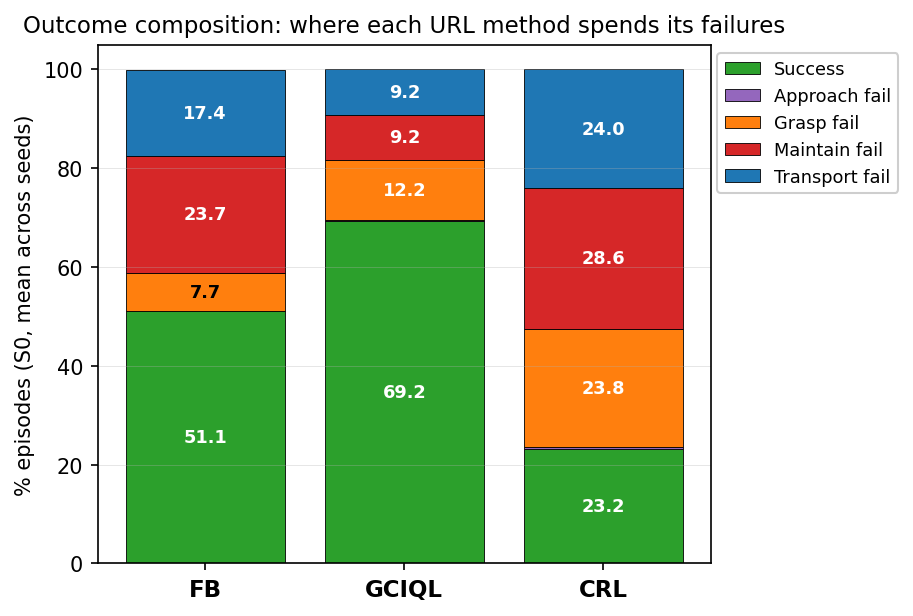
\includegraphics[width=0.72\linewidth]{f3_failure_composition}
\caption{Outcome composition across URL families on \task{} state observations: \fb{} concentrates failure in maintain and transport, \gciql{} is broadly competent with no dominant failure mode, and \crl{}+FlowBC fails broadly across grasp, maintain, and transport. The three failure profiles fall on the same contact-dependent phases, supporting phase-conditioned controllability as the missing representational ingredient. \crl{}+FlowBC is reported from $10$ seeds at the last available checkpoint per seed; the same 4-bucket protocol applies unchanged.}
\label{fig:composition}
\end{figure}

For \crl{}+FlowBC the empirical picture is now in hand and is broader than \fb{}'s post-pick-up profile: grasp failures alone are $3.1\times$ \fb{}'s rate, and the method also drops a substantial fraction of episodes during maintain and transport. A pre-grasp intervention does not rescue \crl{} either (\crl{}+FlowBC secured rate under S2 falls to $58.0\%$ vs.~\fb{}'s $85.1\%$), suggesting the flow-matching actor is implicated in maintain-phase instability independently of the contrastive value. Further representational probes for \crl{} --- in particular, whether future-random separation in the contrastive embedding differs across pre-grasp, lifted, dropped, and transport states --- are left to follow-up work. For \psm{}, the key test is basis coverage: whether any proto-policy or proto-basis assigns substantial successor mass to stable grasped transport. For a model-based method, the key test is phase-transition prediction: whether the learned model predicts contact acquisition, lift, slip, and drop transitions accurately enough to support imagined control.

\bibliographystyle{plainnat}
\bibliography{lib}

\end{document}